\documentclass{article}
\usepackage[utf8]{inputenc}

% Page setup
\usepackage[a4paper,landscape,margin=2cm]{geometry}
\usepackage{amsmath}

% Typography
\usepackage[scaled]{helvet}
\let\familydefault\sfdefault

\usepackage[usenames,svgnames]{xcolor}
\usepackage{tikz,pgfplots}
\usetikzlibrary{positioning,arrows,intersections,calc}

\definecolor{colorwhite}    {RGB}{255,255,255}
\definecolor{colorpod}      {RGB}{199,212,104}
\definecolor{colorfile}     {RGB}{ 79,142,209}
\definecolor{colorsummary}  {RGB}{143,232,186}
\definecolor{colortext}     {RGB}{ 29, 29, 27}
\definecolor{colorkey}      {RGB}{129, 29, 27}
\definecolor{colorclient}   {RGB}{190, 22, 34}

\begin{document}
\pagestyle{empty}
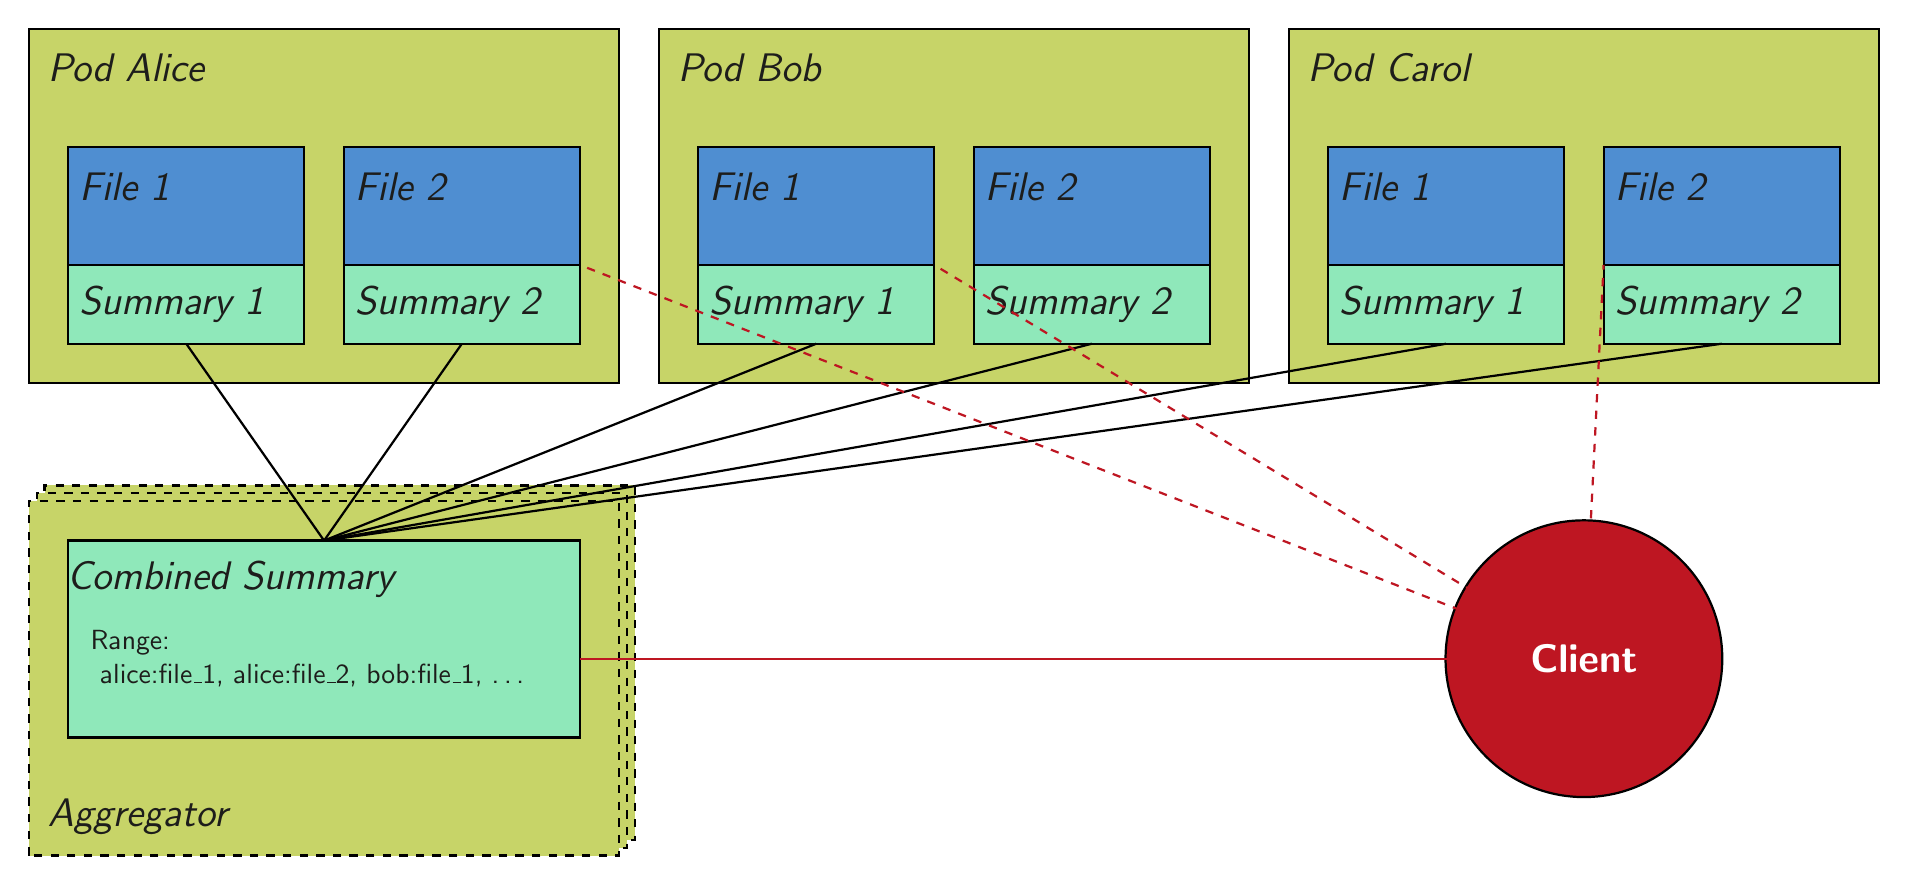
\begin{tikzpicture}[
    node distance = 10em, auto, thick,
    title/.style={text=colortext,font={\Large\itshape}},
    person/.style={text=colorwhite,font={\Large\bfseries}},
    code/.style={text=colortext,font={}},
    key/.style={text=colorkey,font={\tiny\itshape}}
]

    % Pod Alice
    \draw[fill=colorpod] (5.5,1) rectangle (13,5.5);
    \node[title,text width=10em] at (7.5,5) {Pod Alice};
    \draw[fill=colorfile] (6,2.5) rectangle (9,4);
    \node[title,text width=10em] at (7.9,3.5) {File 1};
    \draw[fill=colorsummary] (6,1.5) rectangle (9,2.5);
    \node[title,text width=10em] at (7.9,2) {Summary 1};
    \draw[fill=colorfile] (9.5,2.5) rectangle (12.5,4);
    \node[title,text width=10em] at (11.4,3.5) {File 2};
    \draw[fill=colorsummary] (9.5,1.5) rectangle (12.5,2.5);
    \node[title,text width=10em] at (11.4,2) {Summary 2};
    
    % Pod Bob
    \draw[fill=colorpod] (13.5,1) rectangle (21,5.5);
    \node[title,text width=10em] at (15.5,5) {Pod Bob};
    \draw[fill=colorfile] (14,2.5) rectangle (17,4);
    \node[title,text width=10em] at (15.9,3.5) {File 1};
    \draw[fill=colorsummary] (14,1.5) rectangle (17,2.5);
    \node[title,text width=10em] at (15.9,2) {Summary 1};
    \draw[fill=colorfile] (17.5,2.5) rectangle (20.5,4);
    \node[title,text width=10em] at (19.4,3.5) {File 2};
    \draw[fill=colorsummary] (17.5,1.5) rectangle (20.5,2.5);
    \node[title,text width=10em] at (19.4,2) {Summary 2};
    
    % Pod Carol
    \draw[fill=colorpod] (21.5,1) rectangle (29,5.5);
    \node[title,text width=10em] at (23.5,5) {Pod Carol};
    \draw[fill=colorfile] (22,2.5) rectangle (25,4);
    \node[title,text width=10em] at (23.9,3.5) {File 1};
    \draw[fill=colorsummary] (22,1.5) rectangle (25,2.5);
    \node[title,text width=10em] at (23.9,2) {Summary 1};
    \draw[fill=colorfile] (25.5,2.5) rectangle (28.5,4);
    \node[title,text width=10em] at (27.4,3.5) {File 2};
    \draw[fill=colorsummary] (25.5,1.5) rectangle (28.5,2.5);
    \node[title,text width=10em] at (27.4,2) {Summary 2};
    
    % Aggregator
    \draw[fill=colorpod,dashed] (5.7,-4.8) rectangle (13.2,-0.3);
    \draw[fill=colorpod,dashed] (5.6,-4.9) rectangle (13.1,-0.4);
    \draw[fill=colorpod,dashed] (5.5,-5) rectangle (13,-0.5);
    \node[title,text width=10em] at (7.5,-4.5) {Aggregator};
    \draw[fill=colorsummary] (6,-3.5) rectangle (12.5,-1);
    \node[title,text width=20em] at (9.5,-1.5) {Combined Summary};
    \node[code,text width=20em] at (9.8,-2.5) {Range:\\ \ alice:file\_1, alice:file\_2, bob:file\_1, \ldots};
    
    % Arrows between summaries
    \draw[-,thick](7.5,1.5) to (9.25,-1);
    \draw[-,thick](11,1.5) to (9.25,-1);
    \draw[-,thick](15.5,1.5) to (9.25,-1);
    \draw[-,thick](19,1.5) to (9.25,-1);
    \draw[-,thick](23.5,1.5) to (9.25,-1);
    \draw[-,thick](27,1.5) to (9.25,-1);
    
    % Client
    \draw[fill=colorclient] (25.25,-2.5) circle (50pt);
    \node[person] at (25.25,-2.5) (client) {Client};
    
    % Arrows from client to summary and files
    \draw[-,thick,colorclient] (client) -- (12.5,-2.5);
    \draw[-,thick,dashed,colorclient] (client) -- (12.5,2.5);
    \draw[-,thick,dashed,colorclient] (client) -- (17,2.5);
    \draw[-,thick,dashed,colorclient] (client) -- (25.5,2.5);

\end{tikzpicture}
\end{document}
